\documentclass{standalone}
  \usepackage{tikz}
  \usetikzlibrary{arrows.meta, automata, bending, positioning, shapes.misc}
  \tikzstyle{automaton}=[shorten >=1pt, >={Stealth[bend,round]}, initial text=]
  \tikzstyle{accepting}=[accepting by arrow]

\begin{document}
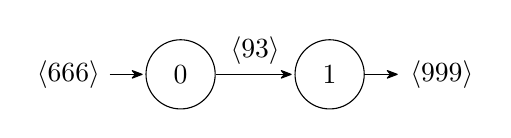
\begin{tikzpicture}[automaton, auto]
  \node[state,initial,initial text=$\left\langle 666\right\rangle$] (0) {$0$};
  \node[state,accepting,accepting text=$\left\langle 999\right\rangle$] (1) [right=of 0] {$1$};
  \path[->] (0) edge node {$\left\langle 93\right\rangle $} (1);
\end{tikzpicture}
\end{document}
